\documentclass[11pt,a4paper]{article}

\usepackage[margin=1in]{geometry}
\usepackage{amsmath}
\usepackage{amssymb}
\usepackage{array}
\usepackage{booktabs}
\usepackage{enumitem}
\usepackage{float}
\usepackage{graphicx}
\usepackage{hyperref}
\usepackage{longtable}
\usepackage{xcolor}
\usepackage{listings}
\usepackage{caption}
\usepackage{subcaption}
\usepackage{tabularx}

\graphicspath{{figures/}}

\hypersetup{
    colorlinks=true,
    linkcolor=blue,
    urlcolor=blue,
    citecolor=blue,
    pdftitle={AI Fundamentals Project Portfolio},
    pdfauthor={Mohammad Saleh Mahdinejad and Fatemeh Sayadzadeh}
}

\definecolor{codebg}{RGB}{248,248,248}
\definecolor{codeborder}{RGB}{210,210,210}
\definecolor{darkblue}{RGB}{20,55,95}

\lstset{
    basicstyle=\ttfamily\small,
    backgroundcolor=\color{codebg},
    breaklines=true,
    frame=single,
    rulecolor=\color{codeborder},
    columns=fullflexible,
    showstringspaces=false,
    tabsize=4
}

\newcommand{\code}[1]{\texttt{#1}}

\begin{document}

\begin{titlepage}
    \centering
    \vspace*{1.2cm}
    {\Large Fundamentals and Applications of Artificial Intelligence\par}
    \vspace{1.0cm}
    {\Huge\bfseries AI Fundamentals Project Portfolio\par}
    \vspace{0.4cm}
    {\Large Search, Learning, Decision Making, Games, Logic, and LLM-Symbolic Reasoning\par}
    \vspace{1.5cm}
    \begin{tabular}{rl}
        \textbf{Team Members:} & Mohammad Saleh Mahdinejad \\
                               & Fatemeh Sayadzadeh \\
        \textbf{Repository:}   & \code{AI\_Fundamentals} \\
        \textbf{Document Type:} & Consolidated technical report \\
    \end{tabular}
    \vfill
    {\large \today\par}
\end{titlepage}

\begin{abstract}
This report documents a consolidated portfolio of five artificial intelligence course projects. The projects begin with classical graph search and optimization, continue through regression, local search, Markov decision processes, reinforcement learning, and adversarial games, and end with first-order logic and hybrid LLM-symbolic reasoning. The final repository was built by reviewing the original assignment repositories, preserving the executable code and required assets, removing classroom metadata and temporary artifacts, cleaning sensitive configuration, and writing a single professional documentation layer around the complete body of work.
\end{abstract}

\tableofcontents
\newpage

\section{Introduction}

The purpose of this repository is to present the full output of the AI fundamentals course as one coherent portfolio rather than as five isolated classroom repositories. Each original repository focused on a different family of AI methods:

\begin{itemize}[leftmargin=*]
    \item deterministic and informed search,
    \item numerical learning and gradient-based optimization,
    \item stochastic decision making and reinforcement learning,
    \item adversarial search for competitive games,
    \item symbolic inference using first-order logic,
    \item and hybrid reasoning where an LLM generates constraints validated by a symbolic solver.
\end{itemize}

The final repository keeps the phases independent enough to run separately, but it also creates one shared README, one shared dependency file, and this report as the main explanation of the implementation.

\subsection{Source Material Reviewed}

The consolidated report is based on both the code and the phase documents that were part of the original repositories. The following table summarizes the reviewed material.

\begin{longtable}{p{0.28\textwidth}p{0.30\textwidth}p{0.32\textwidth}}
\toprule
\textbf{Original Repository} & \textbf{Reviewed Documents} & \textbf{Main Code/Notebook Artifacts} \\
\midrule
\endhead
\code{search-regression-annealing-star} & \code{phase1-doc.pdf}, \code{Report.pdf} & BFS/UCS/DLS/A* scripts, regression notebook, DNA center notebook \\
\code{mdp-unknown-star} & \code{phase2-doc.pdf}, \code{phase2-env-instruction.pdf} & MDP solver, Q-learning solver, DQN bonus implementation \\
\code{game-star} & \code{phase3.pdf} & PaintBattle environment, minimax agent, maps, binary enemy agents \\
\code{fol-star} & \code{phase4.pdf} & Minesweeper environment, PyDatalog solver, manual controller \\
\code{fol-llm-star} & \code{phase4-bonus.pdf} & Mastermind environment, LLM-Prolog solver, manual game \\
\bottomrule
\end{longtable}

\subsection{Final Repository Structure}

\begin{lstlisting}
AI_Fundamentals/
  README.md
  requirements.txt
  docs/
    AI_Fundamentals_Report.tex
    AI_Fundamentals_Report.pdf
    figures/
  projects/
    phase-01-search-regression-annealing/
    phase-02-mdp-reinforcement-learning/
    phase-03-adversarial-search-game/
    phase-04-fol-minesweeper/
    phase-05-llm-fol-mastermind/
\end{lstlisting}

\section{Phase 1: Search, Regression, and Local Search}

\subsection{Scope}

Phase 1 contains three independent tasks. The first task is a grid-world search problem based on an Angry Birds style environment. The second task predicts asteroid diameter with a linear regression model trained by stochastic gradient descent implemented from scratch. The third task solves the closest DNA string problem using local search algorithms.

\subsection{Part A: Grid Search}

\subsubsection{Problem Definition}

The search environment is implemented in \code{search\_algorithms/env/env.py}. The agent moves through a grid containing grass, bushes, rocks, targets, and an enemy following a periodic path. The objective is to collect all targets while avoiding collisions and minimizing unnecessary exploration. The environment exposes the search interface through methods such as:

\begin{itemize}[leftmargin=*]
    \item \code{get\_successors()} for valid next states and costs,
    \item \code{is\_goal\_state()} for target completion,
    \item \code{is\_collision\_state()} for enemy and obstacle collisions,
    \item \code{get\_enemy\_path()} and \code{get\_enemy\_position()} for dynamic enemy reasoning,
    \item \code{get\_targets\_positions()} for remaining goals.
\end{itemize}

The environment uses non-uniform costs: grass is cheap, bushes are expensive, rocks block movement, target collection increases score, and enemy collision is heavily penalized. The scoring environment therefore rewards both correctness and efficiency.

\subsubsection{State Representation}

A key design decision in the implemented search algorithms is that a visited state is not represented only by the agent position. The enemy position changes with time, and target collection changes future goals. The implemented state key therefore includes:

\begin{equation}
    state\_key = (agent\_position,\ remaining\_targets,\ enemy\_cycle\_step)
\end{equation}

This prevents a common bug in dynamic environments: pruning a position as visited even though it occurs at a different time step with a different enemy location.

\subsubsection{BFS}

\code{BFS\_main.py} implements breadth-first search with a FIFO queue. It is suitable when edge costs are uniform and the primary objective is minimum number of actions. The implementation stores a path beside each frontier state and returns the path when \code{is\_goal\_state()} is reached. Collision states are skipped before insertion into the frontier.

A second version, \code{bfs\_with\_wait}, introduces an explicit wait-like behavior in blocked enemy situations. It compares normal successors with successors that include wall-directed actions and uses \code{is\_enemy\_blocking()} to decide whether waiting is necessary to avoid an immediate trap.

\subsubsection{UCS}

\code{UCS\_main.py} uses a priority queue ordered by cumulative path cost \(g(n)\). This is necessary because bush and grass movement costs are different. UCS expands the cheapest frontier node first and stores the best known cost for each state key:

\begin{equation}
    g(n) = \sum_{i=1}^{k} cost(a_i)
\end{equation}

The implementation uses \code{heapq}, a monotonically increasing counter for tie-breaking, and a dictionary of visited costs to avoid discarding a cheaper path that reaches the same logical state later.

\subsubsection{DLS and IDS}

\code{DLS\_main.py} implements recursive depth-limited search and wraps it inside iterative deepening search. Depth-limited search is memory efficient, but it can miss solutions deeper than the chosen limit. IDS solves that by increasing the limit gradually:

\begin{equation}
    limit = 0, 1, 2, \ldots, max\_depth
\end{equation}

The implementation includes both standard and wait-aware variants. The wait-aware version mirrors the BFS logic and adds staying behavior only when the enemy blocks safe progress.

\subsubsection{A*}

\code{AStar\_main.py} implements an informed search strategy. The heuristic is built from:

\begin{itemize}[leftmargin=*]
    \item Manhattan distance from the agent to targets,
    \item an obstacle-aware weighted distance,
    \item a minimum spanning tree style estimate over remaining targets,
    \item and a penalty for proximity to enemies.
\end{itemize}

The heuristic structure can be summarized as:

\begin{equation}
    f(n) = g(n) + h(n)
\end{equation}

where \(h(n)\) estimates the cost of collecting remaining targets. The implementation decomposes the problem by searching to the next target, updating the current state, and continuing until all targets are collected. This greedy decomposition keeps the search tractable on harder maps while still benefiting from the heuristic.

\subsection{Part B: Linear Regression with SGD}

\subsubsection{Task}

The regression notebook, \code{linear\_regression/modeling\_hint.ipynb}, predicts asteroid diameter using orbital and physical features. The original assignment required preprocessing, exploratory data analysis, and a custom implementation of stochastic gradient descent rather than simply calling a ready-made scikit-learn regressor.

\subsubsection{Data Pipeline}

The notebook uses:

\begin{itemize}[leftmargin=*]
    \item \code{pandas} for tabular loading and cleaning,
    \item \code{numpy} for vectorized numerical operations,
    \item \code{matplotlib} and \code{seaborn} for visualization,
    \item \code{StandardScaler} and \code{LabelEncoder} for preprocessing,
    \item train/validation/test splits for evaluation and early stopping.
\end{itemize}

The final feature matrix contains numeric and encoded categorical features. Scaling is important because SGD is sensitive to feature magnitude; unscaled features would make gradient steps unstable or force a much smaller learning rate.

\subsubsection{Model}

The implemented model is a scratch linear regressor. For input vector \(x_i\), prediction is:

\begin{equation}
    \hat{y_i} = w^T x_i + b
\end{equation}

The training objective is mean squared error:

\begin{equation}
    MSE = \frac{1}{n}\sum_{i=1}^{n}(y_i - \hat{y_i})^2
\end{equation}

The weight update follows stochastic gradient descent with optional improvements such as momentum, learning-rate decay, and early stopping:

\begin{equation}
    w \leftarrow w - \alpha \nabla_w MSE
\end{equation}

\subsubsection{Evaluation}

The notebook evaluates the trained model using \(R^2\), MAE, and MSE. The original report records a final training loss around \(0.001069\), and the prediction plots show \(R^2\) values around \(0.927\), which passes the assignment target of \(R^2 \geq 0.8\).

\begin{figure}[H]
    \centering
    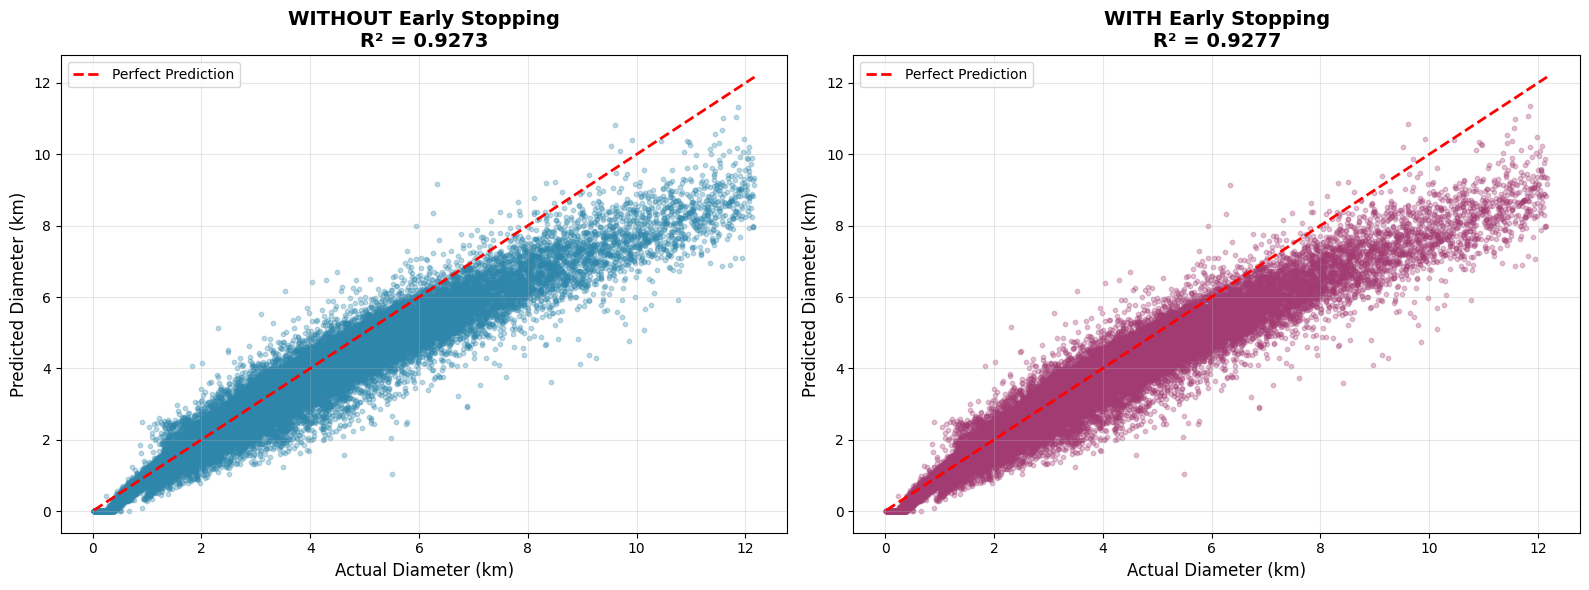
\includegraphics[width=0.95\textwidth]{phase1_regression_early_stopping.png}
    \caption{Comparison of regression predictions with and without early stopping.}
\end{figure}

\begin{figure}[H]
    \centering
    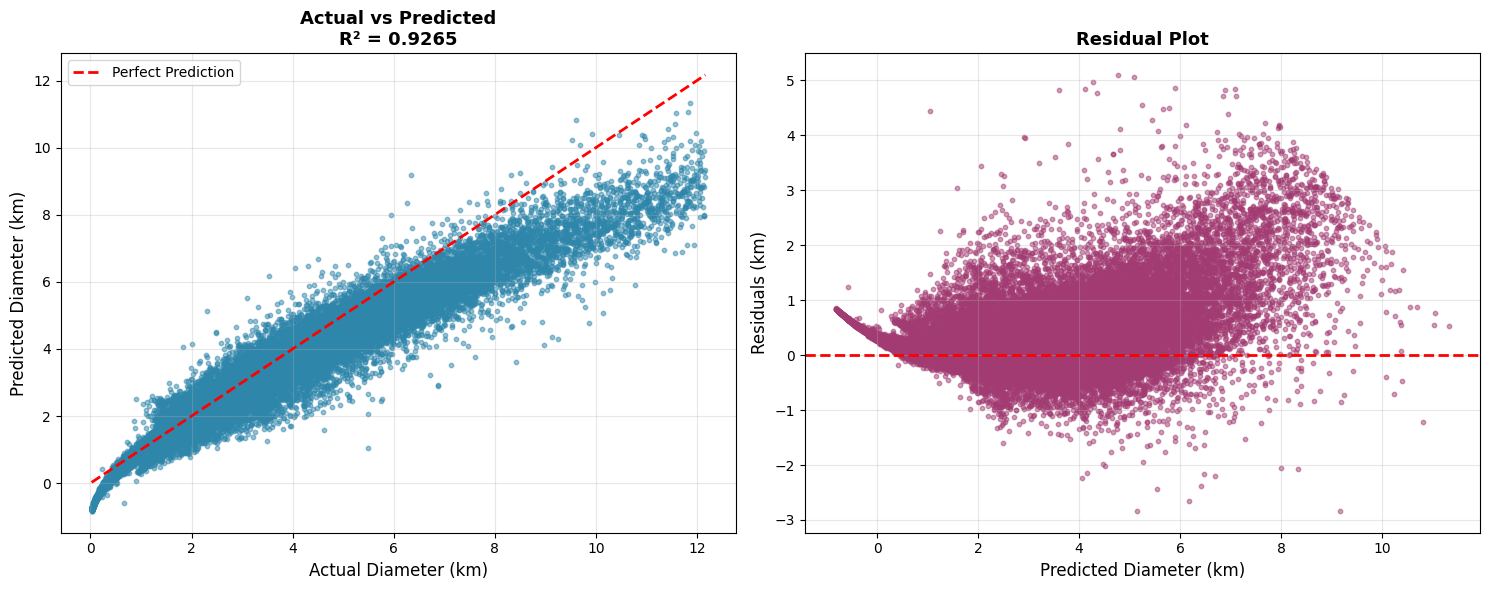
\includegraphics[width=0.95\textwidth]{phase1_regression_residuals.png}
    \caption{Actual-vs-predicted and residual analysis for the asteroid diameter model.}
\end{figure}

\subsection{Part C: DNA Center Finding}

\subsubsection{Problem Definition}

The DNA task is a closest string problem. Given a set of DNA strings with equal length, the goal is to find a center string minimizing the largest Hamming distance to the input set:

\begin{equation}
    \min_{s \in \{A,C,G,T\}^L}\ \max_{x \in X} d_H(s, x)
\end{equation}

The evaluation function is therefore:

\begin{equation}
    f(s) = \max_{x \in X} d_H(s, x)
\end{equation}

\subsubsection{Implemented Local Search Methods}

The notebook \code{simulated\_annealing/DNA\_Center.ipynb} implements the required functions for state initialization, evaluation, neighbor generation, and local search. The implementation compares:

\begin{itemize}[leftmargin=*]
    \item hill climbing,
    \item random-restart hill climbing,
    \item stochastic hill climbing,
    \item random-walk hill climbing,
    \item simulated annealing,
    \item and brute force for small instances.
\end{itemize}

Hill climbing always moves to a better neighbor and can become stuck in local minima. Simulated annealing can temporarily accept worse states according to:

\begin{equation}
    P(accept) = e^{-\Delta/T}
\end{equation}

where \(\Delta\) is the increase in cost and \(T\) is the temperature. This makes annealing more robust on rugged search spaces.

\begin{figure}[H]
    \centering
    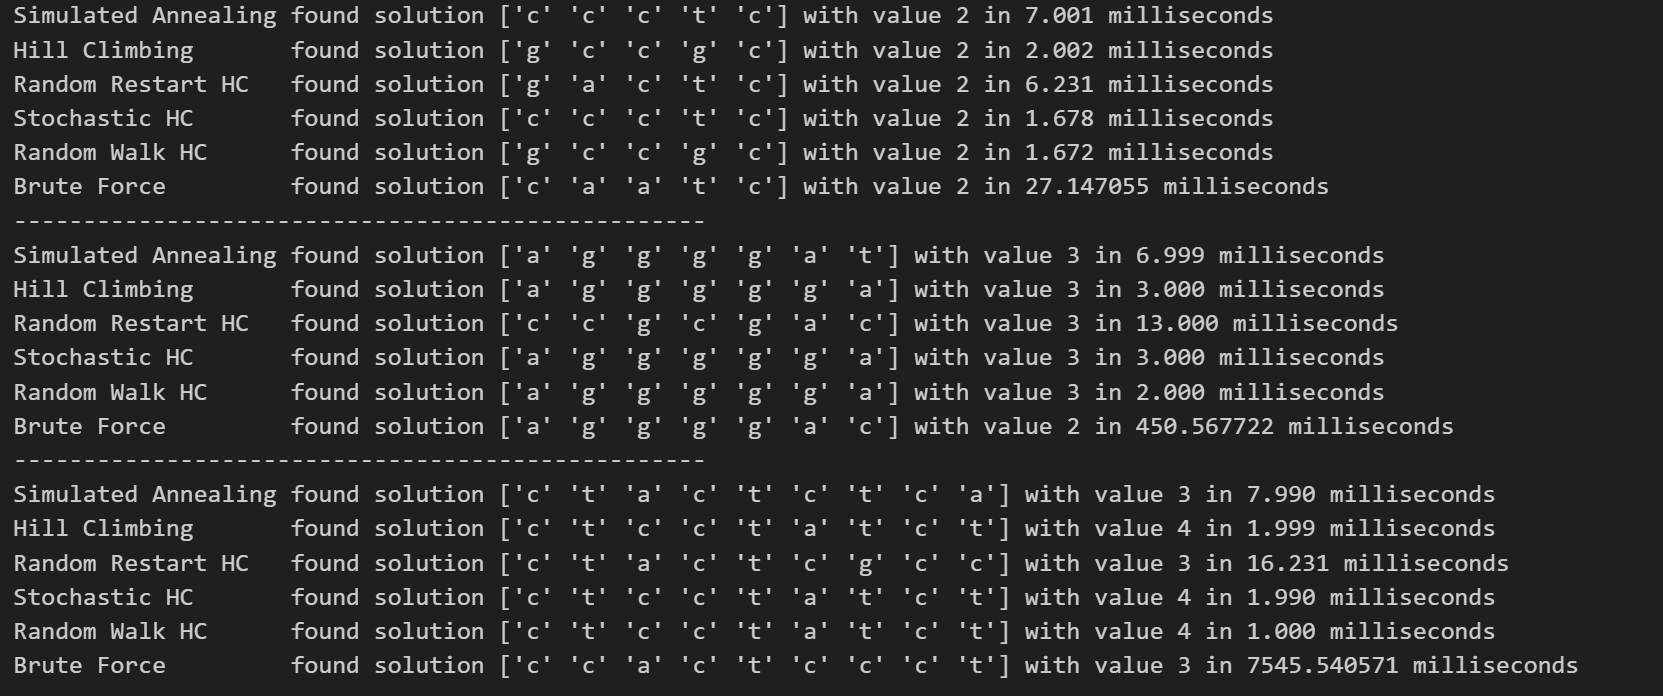
\includegraphics[width=0.92\textwidth]{phase1_dna_results.png}
    \caption{Extracted comparison output for DNA center search methods.}
\end{figure}

\section{Phase 2: MDP and Reinforcement Learning}

\subsection{Scope}

Phase 2 studies a stochastic WALL-E environment. The phase is split into a known-environment MDP solver, an unknown-environment Q-learning solver, and a DQN bonus.

\subsection{Environment}

The main grid is \(8 \times 8\). WALL-E starts at the upper-left corner and must reach the plant while collecting trash, avoiding buildings and enemies, and respecting a maximum number of actions. Actions are stochastic: when the agent selects a direction, the actual movement may follow the intended direction or one of its neighboring directions according to a fixed transition distribution created for the environment.

Important rewards and penalties include:

\begin{itemize}[leftmargin=*]
    \item goal reward: \(+400\),
    \item default movement reward: \(-1\),
    \item enemy collision: \(-400\),
    \item trash collection reward: \(+250\) in the fully collectable case,
    \item limited action budget, usually 150 moves.
\end{itemize}

\begin{figure}[H]
    \centering
    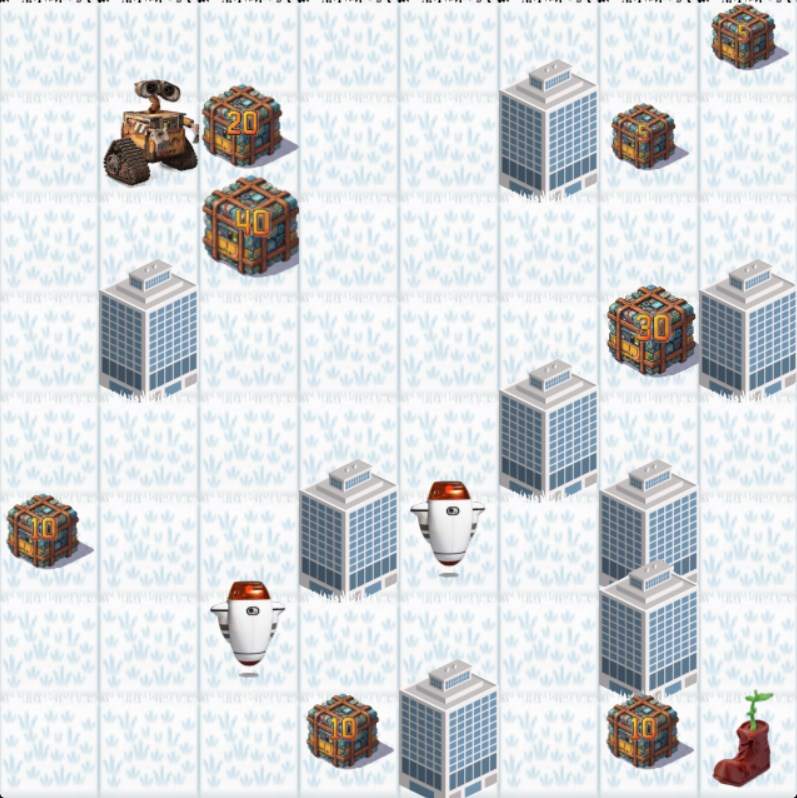
\includegraphics[width=0.70\textwidth]{phase2_mdp_environment.png}
    \caption{Known-environment WALL-E grid with buildings, trash, enemies, and goal.}
\end{figure}

\subsection{Known Environment: Value Iteration}

\subsubsection{Transition Model}

The known MDP solver uses the transition model exposed by the environment. For each state-action pair, the model enumerates possible next states, probabilities, and rewards. The value iteration update is:

\begin{equation}
    V_{k+1}(s) = \max_a \sum_{s'} P(s' \mid s,a)\left[R(s,a,s') + \gamma V_k(s')\right]
\end{equation}

The implemented solver uses \(\gamma = 0.99\), a small convergence threshold, and up to 5000 iterations.

\subsubsection{Reward Maps}

The project does not rely on a single static reward map. Instead, \code{mdp/main.py} builds multiple reward maps:

\begin{itemize}[leftmargin=*]
    \item \code{build\_reward\_map\_for\_goal}: emphasizes reaching the plant safely,
    \item \code{build\_reward\_map\_for\_trash}: targets a specific trash item,
    \item \code{build\_reward\_map\_for\_collection}: encourages general collection based on current power threshold.
\end{itemize}

The policy therefore depends on a meta-state, especially the current power threshold. A trash item with value 40 should not be treated the same when WALL-E has power 5 and when it has power 40.

\subsubsection{Policy Selection}

After precomputing policies, the execution loop uses \code{select\_optimal\_policy}. This policy selector considers:

\begin{itemize}[leftmargin=*]
    \item remaining moves,
    \item distance to the goal,
    \item accessible trash,
    \item risk around enemies,
    \item current power threshold,
    \item stuck detection based on recent position history.
\end{itemize}

This architecture separates expensive planning from real-time execution. Value iteration runs before play, while the policy selector picks the relevant precomputed policy during play.

\subsubsection{Visualization}

The solver saves heat maps and convergence curves for goal, trash, and collection policies. This was part of the phase requirement and helps inspect whether value iteration is converging and whether the learned value surface makes sense.

\subsection{Unknown Environment: Q-Learning}

\subsubsection{Problem Changes}

In the unknown environment, the agent does not know the reward or transition model in advance. It must learn from interaction. The state is richer than position alone:

\begin{equation}
    s = (position,\ power\_level,\ trash\_mask)
\end{equation}

The \code{trash\_mask} compresses remaining trash information into a bitmask. The implementation lazily initializes Q-values only when a state is encountered.

\begin{figure}[H]
    \centering
    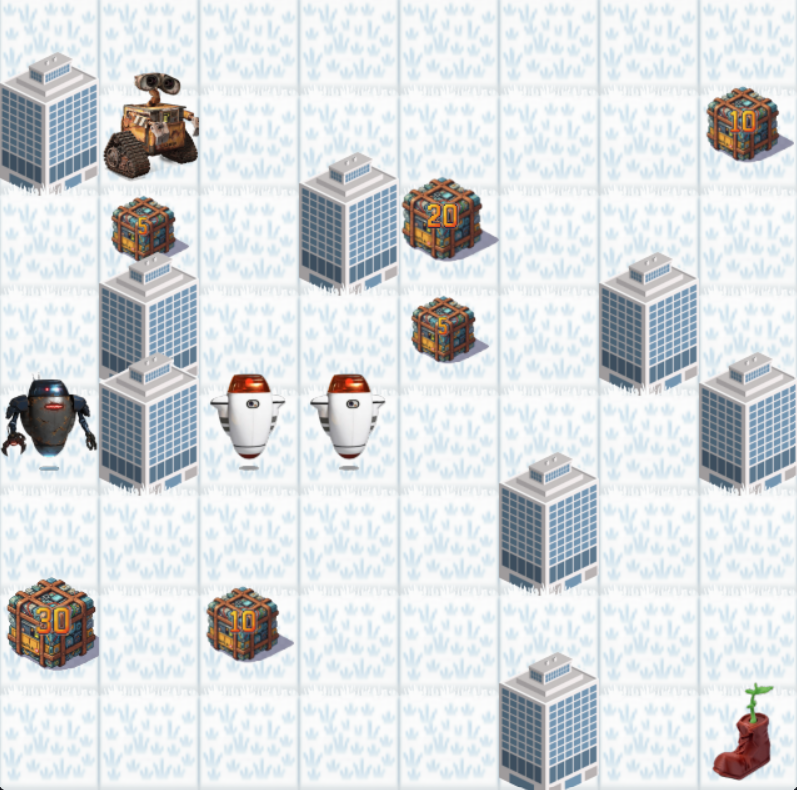
\includegraphics[width=0.70\textwidth]{phase2_unknown_environment.png}
    \caption{Unknown-environment variant with hunter, enemies, buildings, trash, and goal.}
\end{figure}

\subsubsection{Q-Learning Update}

The agent applies the standard Q-learning update:

\begin{equation}
    Q(s,a) \leftarrow Q(s,a) + \alpha \left[r + \gamma \max_{a'}Q(s',a') - Q(s,a)\right]
\end{equation}

The implemented parameters include learning-rate decay, epsilon decay, a minimum epsilon, and a minimum learning rate. Training is configured for 30,000 episodes. Every 1000 episodes, the code records a value-difference metric by comparing the current and previous Q-tables.

\subsubsection{Evaluation}

After training, the script tests the greedy policy, saves a convergence plot, generates a policy map for a reference state, and writes a summary file. The grading thresholds from the phase document focus on mean score, with higher scores corresponding to stronger learned behavior.

\subsection{Bonus: Dueling DQN}

The DQN bonus uses PyTorch to approximate Q-values with a neural network. The implemented architecture is dueling:

\begin{equation}
    Q(s,a) = V(s) + A(s,a) - \frac{1}{|\mathcal{A}|}\sum_{a'} A(s,a')
\end{equation}

The agent includes:

\begin{itemize}[leftmargin=*]
    \item a policy network and target network,
    \item replay buffer,
    \item mini-batch training,
    \item target-network synchronization,
    \item epsilon-greedy action selection,
    \item vector state representation with position, power, and trash state.
\end{itemize}

The bonus environment is smaller and simplified compared with the full \(8 \times 8\) environment, which makes neural training more practical.

\section{Phase 3: Adversarial Search Game}

\subsection{Environment}

The PaintBattle project implements a competitive two-player grid game. Each player moves across a map and paints territory. Capturing enclosed regions can change the score quickly, so a locally good move may be bad after the opponent responds. This makes the project a natural adversarial search problem.

The main environment is \code{src/env.py}. It defines:

\begin{itemize}[leftmargin=*]
    \item \code{PBState}: immutable-style state container for grid, paint matrix, player positions, step count, and alive flags,
    \item \code{get\_successors(team)}: valid successor generation for a team,
    \item \code{capture\_logic}: local region capture behavior,
    \item \code{get\_scores}: territory scoring,
    \item \code{PaintBattle.play}: full Pygame loop for two agents.
\end{itemize}

\subsection{Agent Interface}

Every player inherits from the base \code{Agent} class and implements:

\begin{lstlisting}[language=Python]
def get_action(self, state):
    raise NotImplementedError
\end{lstlisting}

The final AI agent is \code{MinimaxAgent} in \code{Minimax1.py}. In \code{main.py}, it is configured with depth 9 and played against packaged binary enemy agents.

\subsection{Map Example}

\begin{lstlisting}
GGGGGGGGG1
GGGGGGGGGG
GGGGGGGGGG
GGGGGGGGGG
GGGGGGGGGG
GGGGGGGGGG
GGGGGGGGGG
GGGGGGGGGG
GGGGGGGGGG
2GGGGGGGGG
\end{lstlisting}

Here, \code{G} represents normal ground and \code{1}/\code{2} mark player start positions. Other maps introduce blocked regions with \code{R}.

\subsection{Minimax with Alpha-Beta Pruning}

The minimax tree alternates between maximizing the controlled agent's utility and minimizing it under the opponent's best response. The recursive value is:

\begin{equation}
    minimax(s,d) =
    \begin{cases}
        eval(s), & d=0 \text{ or terminal}(s) \\
        \max_{s' \in Succ(s)} minimax(s', d-1), & \text{max turn} \\
        \min_{s' \in Succ(s)} minimax(s', d-1), & \text{min turn}
    \end{cases}
\end{equation}

Alpha-beta pruning avoids branches that cannot affect the final decision:

\begin{equation}
    \alpha = \max(\alpha, v),\quad \beta = \min(\beta, v),\quad \alpha \geq \beta \Rightarrow prune
\end{equation}

\subsection{Heuristic Evaluation}

The game is usually not searched until a terminal state, so evaluation quality matters. The implemented \code{evaluate} function combines:

\begin{itemize}[leftmargin=*]
    \item score difference between teams,
    \item alive/dead status,
    \item mobility count,
    \item territory control,
    \item distance pressure,
    \item opponent constraints,
    \item and local tactical opportunities.
\end{itemize}

The agent also uses quick move evaluation and move ordering. Better ordering improves alpha-beta effectiveness because good moves raise \(\alpha\) or lower \(\beta\) earlier.

\section{Phase 4: First-Order Logic Minesweeper}

\subsection{Problem}

Minesweeper is a partial-information puzzle. Revealed cells provide numeric clues, hidden cells may contain mines, and the solver must infer safe moves without directly observing mine locations. The phase document required using first-order logic style reasoning through PyDatalog or a Prolog-like engine.

\subsection{Environment}

The environment is implemented in \code{src/minesweeper.py}. It provides:

\begin{itemize}[leftmargin=*]
    \item \code{reveal(r,c)} returning \(-1\) for a mine or a clue from 0 to 8,
    \item \code{flag(r,c)} and \code{unflag(r,c)},
    \item deterministic board generation through a seed,
    \item Pygame rendering and HUD output,
    \item victory detection and mine counting.
\end{itemize}

\begin{figure}[H]
    \centering
    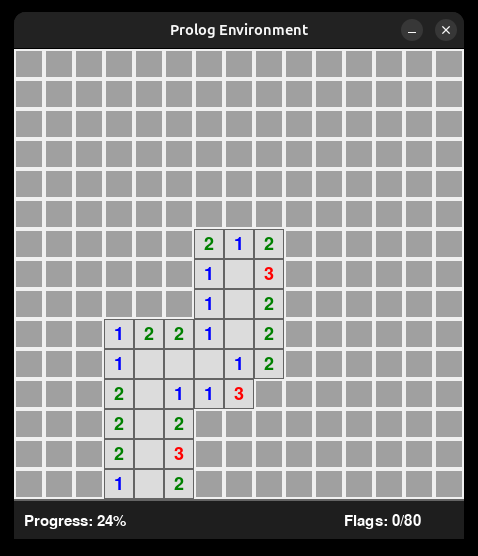
\includegraphics[width=0.48\textwidth]{phase4_minesweeper_solver.png}
    \caption{Extracted solver-state visualization from the Minesweeper phase documentation.}
\end{figure}

\subsection{Knowledge Representation}

The solver in \code{main.py} defines PyDatalog terms:

\begin{itemize}[leftmargin=*]
    \item \code{hidden(R,C)}
    \item \code{revealed(R,C)}
    \item \code{flagged(R,C)}
    \item \code{neighbor(R,C,NR,NC)}
    \item \code{clue(R,C,V)}
    \item \code{flagged\_count(R,C,FC)}
    \item \code{hidden\_count(R,C,HC)}
    \item \code{safe(R,C)}, \code{mine(R,C)}, \code{safe\_zero(R,C)}, \code{frontier(R,C)}
\end{itemize}

Board topology is asserted once at startup. Dynamic facts are updated after each reveal or flag.

\subsection{Inference Rules}

The main safe-cell rule is:

\begin{equation}
    clue(R,C,V) \land flagged\_count(R,C,V) \Rightarrow hidden\ neighbors\ are\ safe
\end{equation}

The main mine rule is:

\begin{equation}
    flagged\_count(R,C,FC) + hidden\_count(R,C,HC) = V \Rightarrow hidden\ neighbors\ are\ mines
\end{equation}

The solver also has a zero-clue rule:

\begin{equation}
    clue(R,C,0) \Rightarrow all\ hidden\ neighbors\ are\ safe
\end{equation}

To reduce unnecessary queries, the solver uses a \code{frontier} predicate: only revealed cells adjacent to at least one hidden cell need to be considered.

\subsection{Control Loop}

Each cycle performs:

\begin{enumerate}[leftmargin=*]
    \item render the board,
    \item compute temporary flagged/hidden neighbor counts,
    \item query \code{safe\_zero}, then \code{safe}, then \code{mine},
    \item batch reveal or flag actions,
    \item retract temporary count facts,
    \item fall back to risk-based guessing if no logical move exists.
\end{enumerate}

The fallback is not pure FOL, but it is necessary because Minesweeper can reach states where deterministic local inference is insufficient.

\section{Phase 5: LLM + FOL Mastermind}

\subsection{Problem}

Mastermind is a code-breaking game. A secret code is generated from an alphabet, and each guess receives three feedback values:

\begin{itemize}[leftmargin=*]
    \item correct: right symbol in the right position,
    \item misplaced: right symbol in the wrong position,
    \item incorrect: symbol not present in the secret.
\end{itemize}

\begin{figure}[H]
    \centering
    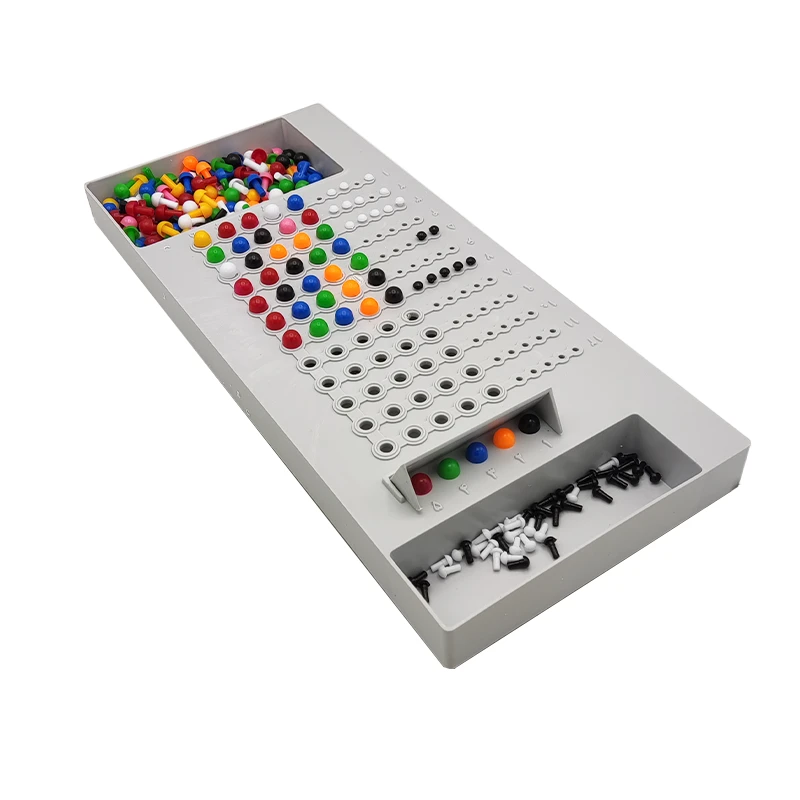
\includegraphics[width=0.55\textwidth]{phase5_mastermind_board.png}
    \caption{Mastermind board image extracted from the original bonus documentation.}
\end{figure}

\subsection{Manual Game}

\code{manual\_game.py} provides a direct interactive version. The default configuration is:

\begin{itemize}[leftmargin=*]
    \item alphabet: \code{ABCDE},
    \item code length: 5,
    \item maximum turns: 12.
\end{itemize}

This file is useful for validating the environment independently of LLM and Prolog dependencies.

\subsection{Logic-LM Architecture}

The bonus document is based on the Logic-LM pattern: natural language models generate symbolic formulations, and a symbolic reasoner checks or solves them. In this project, the LLM is not trusted blindly. Its output is parsed and validated before it becomes part of the Prolog knowledge base.

\begin{figure}[H]
    \centering
    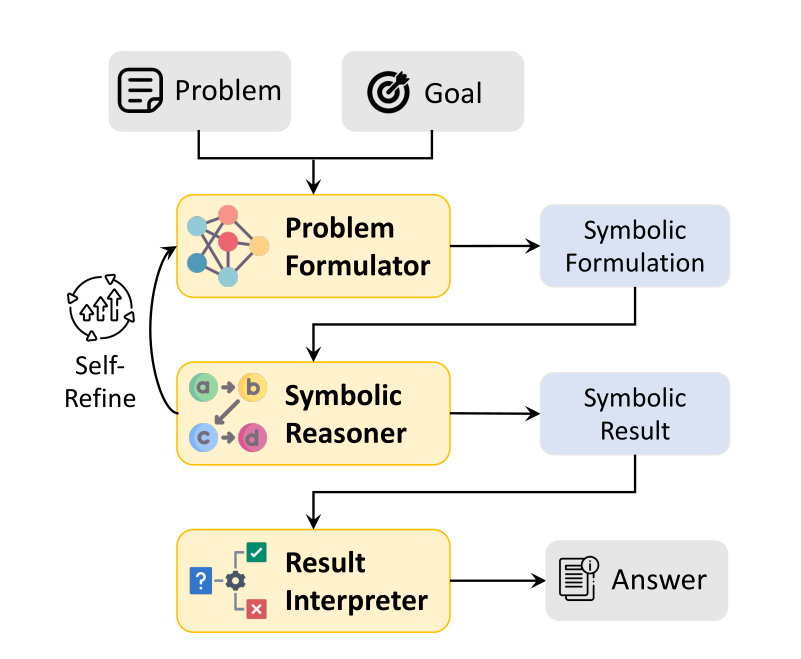
\includegraphics[width=0.72\textwidth]{phase5_logic_lm_architecture.png}
    \caption{Logic-LM architecture from the original bonus phase documentation.}
\end{figure}

\subsection{Generated Prolog Base}

\code{llm\_solver.py} writes \code{logic.pl} dynamically for the selected difficulty. It defines:

\begin{itemize}[leftmargin=*]
    \item the valid alphabet,
    \item code length,
    \item valid-code predicate,
    \item \code{calc\_score/5},
    \item correct-position counting,
    \item removal of exact matches,
    \item misplaced counting through symbol occurrences.
\end{itemize}

The core scoring relation is:

\begin{lstlisting}
calc_score(Secret, Guess, C, M, I) :-
    calc_correct(Secret, Guess, C),
    remove_correct(Secret, Guess, S_Rest, G_Rest),
    calc_misplaced(S_Rest, G_Rest, M),
    code_length(Len),
    I is Len - C - M.
\end{lstlisting}

\subsection{LLM Constraint Generation}

After each guess, the solver asks the LLM to generate a rule like:

\begin{lstlisting}
turn_1(Candidate) :-
    calc_score(Candidate, ['A','B','C','D','E'], 1, 2, 2).
\end{lstlisting}

The implementation validates:

\begin{itemize}[leftmargin=*]
    \item that the rule matches the expected predicate structure,
    \item that the feedback values sum to the code length,
    \item that no feedback value is negative,
    \item that the LLM did not alter the actual feedback values.
\end{itemize}

If validation fails, the code uses a deterministic fallback rule generated by Python. This is an important engineering choice: the LLM helps formulate constraints, but the solver remains robust against hallucinated or malformed output.

\subsection{Candidate Selection}

The \code{PrologSolver} asserts validated constraints and queries:

\begin{lstlisting}
valid_code(C), turn_1(C), turn_2(C), ...
\end{lstlisting}

The resulting candidates are passed back to the LLM for strategic selection when there are multiple possibilities. If the LLM returns an invalid candidate, the code retries and eventually falls back to a random valid candidate. The final implementation also removes hardcoded credentials and reads:

\begin{itemize}[leftmargin=*]
    \item \code{OPENAI\_API\_KEY},
    \item \code{OPENAI\_BASE\_URL},
    \item \code{OPENAI\_MODEL}.
\end{itemize}

\section{Repository Cleanup and Engineering Decisions}

\subsection{Files Preserved}

The final repository preserves:

\begin{itemize}[leftmargin=*]
    \item source code for every phase,
    \item notebooks for regression and DNA center search,
    \item maps and icons required by Pygame environments,
    \item binary enemy agents required by the PaintBattle environment,
    \item LaTeX source and rendered PDF documentation,
    \item phase-level README files.
\end{itemize}

\subsection{Files Removed or Ignored}

The cleanup excludes:

\begin{itemize}[leftmargin=*]
    \item nested \code{.git} directories from source clones,
    \item Python cache directories,
    \item generated training plots and screenshots,
    \item temporary \code{logic.pl},
    \item LaTeX auxiliary files,
    \item hardcoded API credentials.
\end{itemize}

\subsection{Verification}

The consolidated repository was checked with:

\begin{itemize}[leftmargin=*]
    \item Python syntax compilation with \code{python -m compileall projects},
    \item notebook JSON validation,
    \item secret scanning for the previously hardcoded API key pattern,
    \item two-pass LaTeX rendering with \code{pdflatex},
    \item Git status verification after commit and push.
\end{itemize}

\section{Execution Guide}

\subsection{Install Dependencies}

\begin{lstlisting}
python -m venv .venv
.venv\Scripts\activate
pip install -r requirements.txt
\end{lstlisting}

\subsection{Run Phase 1 Search}

\begin{lstlisting}
cd projects/phase-01-search-regression-annealing/search_algorithms
python BFS_main.py
python UCS_main.py
python DLS_main.py
python AStar_main.py
\end{lstlisting}

\subsection{Run Phase 2}

\begin{lstlisting}
cd projects/phase-02-mdp-reinforcement-learning/mdp
python main.py

cd ../unknown_environment
python main.py

cd ../dqn_bonus
python main.py
\end{lstlisting}

\subsection{Run Phase 3}

\begin{lstlisting}
cd projects/phase-03-adversarial-search-game
python main.py
\end{lstlisting}

\subsection{Run Phase 4}

\begin{lstlisting}
cd projects/phase-04-fol-minesweeper
python main.py
\end{lstlisting}

\subsection{Run Phase 5}

\begin{lstlisting}
cd projects/phase-05-llm-fol-mastermind
python manual_game.py

set OPENAI_API_KEY=your_api_key_here
set OPENAI_BASE_URL=https://api.openai.com/v1
set OPENAI_MODEL=gpt-4o-mini
python llm_solver.py
\end{lstlisting}

\section{Conclusion}

This portfolio demonstrates a broad progression across AI methods. Phase 1 starts with deterministic graph search, regression, and local optimization. Phase 2 introduces stochastic transitions, value iteration, tabular reinforcement learning, and neural Q-value approximation. Phase 3 adds competitive reasoning with minimax and alpha-beta pruning. Phase 4 formalizes game knowledge as logical facts and rules. Phase 5 connects modern LLM interfaces to symbolic reasoning through validated Prolog constraints.

The final repository is designed for submission, review, and future extension. It keeps the original implementations intact where they are needed, documents the reasoning behind the algorithms, and provides a clean structure for navigating the complete AI fundamentals project set.

\end{document}
